\documentclass[../../main.tex]{subfiles}
\usepackage{tikz}
\usetikzlibrary{positioning}
\begin{document}
\chapter{Pose Correction for Sign Language Synthesis}
\label{ch:pose_correction}

In the previous chapters, we looked at granularity in sign language animation based on AZee's (linguistic) structure. However, one of the key missing pieces in our study was the ability to shortcut or match a pose on already seen poses. In video games, Motion matching is a technique that dynamically selects the most suitable animation frame or pose from a pre-recorded database based on current input constraints to create fluid, realistic motion. By comparing the motion of the character to a database of motion data, motion matching can generate more realistic and contextually appropriate animations.

The past decade has seen a rise in deep learning technologies in in the field of character animation. These technologies have been used to generate realistic and expressive animations for a wide range of applications, from video games to virtual reality. One of the key challenges in character animation is the generation of natural poses, which requires the ability to capture the nuances of human movement and behavior. 

In this work, we focus on the development of a pose corrector module in our existing synthesis system. We train a pose prior model using a French Sign Language motion capture dataset. The pose prior model captures the typical poses and movements associated with different signs, providing a statistical framework that guides the motion matching process. By learning these priors from a large dataset, our system is able to generate realistic and contextually appropriate sign language poses.

In this chapter, section~\ref{ch:pose_correction:related_work} discusses relevant background work in motion matching and pose correction, focusing on classical methods, data-driven approaches, and the integration of latent space representations. Section~\ref{ch:pose_correction:pose_correction_with_azee} presents the application of thi to the AZee low-level synthesis system, including the preparation of the dataset, training of the Variational Auto Encoder, implementation of pose correction, results and evaluation. Finally, section~\ref{ch:pose_correction:discussion} discusses the implications of integrating pose correction into the AZee system and outlines future directions for research.

\section{Related Work}
\label{ch:pose_correction:related_work}

In this section, we discuss the progression of techniques in generating natural poses for character animation, starting from classical IK methods and moving to modern data-driven approaches. We conclude with the use of pose priors in correcting poses for more realistic outcomes, as used in our sign language animation system.

\subsection{Introduction to Inverse Kinematics (IK)}
\label{ch:pose_correction:related_work:intro_ik}
Inverse Kinematics (IK) is a well-established technique in character animation that computes joint angles to achieve a desired end-effector position. It has found widespread use, but limitations exist, particularly in dynamic and realistic animation contexts.

\subsection{Classical IK Methods and Their Limitations}
\label{ch:pose_correction:related_work:classical_ik}
Classical IK methods, though foundational, face several challenges in handling complex constraints and delivering natural poses in all situations.

\paragraph{Jacobian-Based Methods} Jacobian-based approaches~\cite{4648032} involve calculating the Jacobian matrix to linearize the relationship between joint angles and end-effector positions. By iteratively adjusting joint angles, these methods reduce the error between the current and target positions. Despite their robustness in real-time applications, they suffer from singularities, where solutions become unstable or unrealistic. An example is illustrated in Figure~\ref{fig:jacobian_based}.

\begin{figure}
    \centering 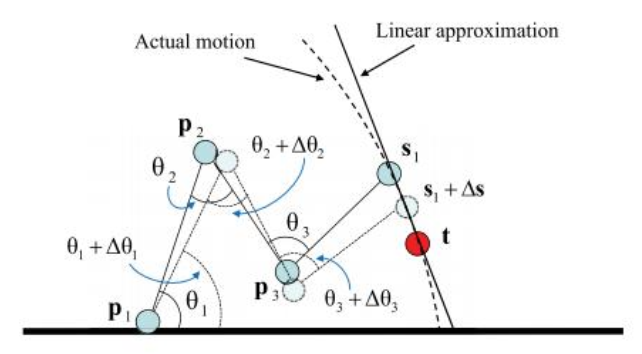
\includegraphics[width = 2.5in]{chapters/pose_correction/images/jacobian_based.png}
    \caption{Jacobian based IK solving (approximation of the first derivative)}
    \label{fig:jacobian_based}
\end{figure}

\paragraph{Cyclic Coordinate Descent (CCD)} CCD~\cite{kenwright2012inverse} simplifies the IK problem by adjusting one joint at a time, minimizing the distance between the end-effector and the target. CCD is computationally efficient and easy to implement, which makes it popular in game engines. However, its greedy approach can lead to suboptimal solutions in more constrained or biomechanically complex setups, as shown in Figure~\ref{fig:ccdik}.

\begin{figure}
  \centering 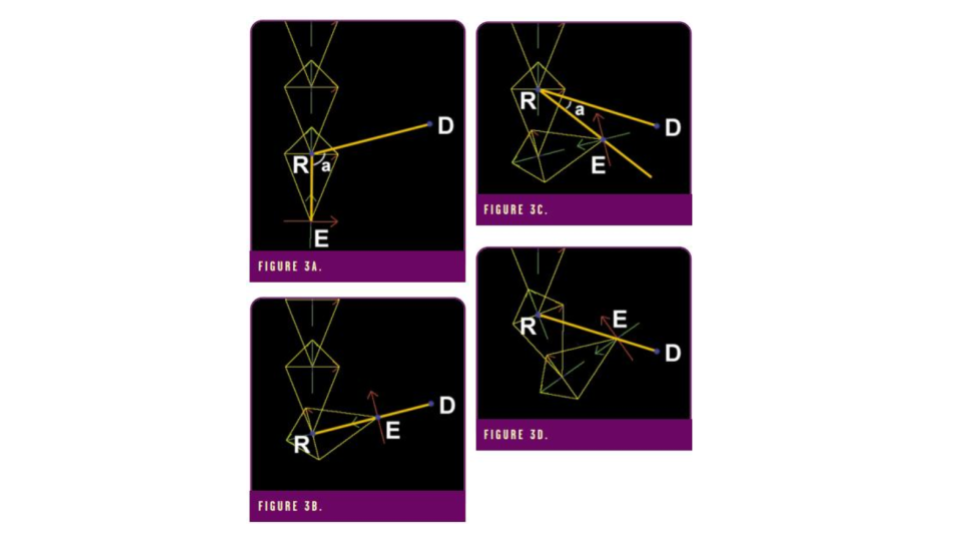
\includegraphics[width = 2.5in]{chapters/pose_correction/images/ccdik.png}
  \caption{Cyclic Coordinate Descent (CCD) IK solving (changes the rotation of a joint, one at a time)}
  \label{fig:ccdik}
\end{figure}

\paragraph{Forward And Backward Reaching Inverse Kinematics (FABRIK)} FABRIK~\cite{aristidou2011fabrik} diverges from other methods by focusing on joint positions rather than angles. It works by iteratively adjusting joint positions in two passes—first from the end-effector to the root, and then from the root to the end-effector. FABRIK is known for its stability and simplicity, particularly in scenarios requiring natural joint configurations, as depicted in Figure~\ref{fig:fabrik}.

\begin{figure}
  \centering 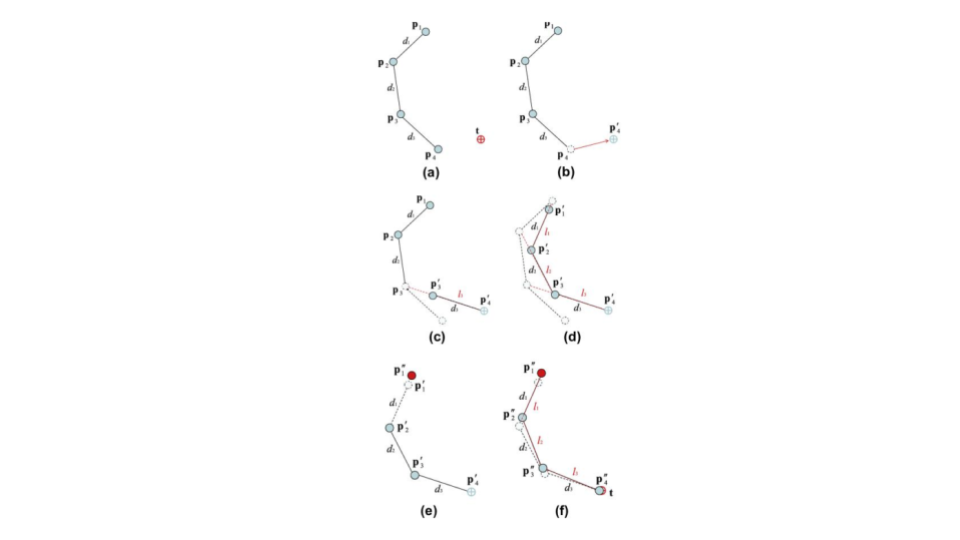
\includegraphics[width = 2.5in]{chapters/pose_correction/images/fabrik.png}
  \caption{Forward And Backward Reaching Inverse Kinematics (FABRIK) solving (updates coordinates in two passes)}
  \label{fig:fabrik}
\end{figure}

\paragraph{Limitations of Classical Methods} These classical IK techniques, while computationally efficient, are prone to singularities, have limited support for complex joint constraints, and often result in unnatural or biomechanically unrealistic poses. As demonstrated in Figure~\ref{fig:problems_classical}, they struggle with overlapping chains and handling multiple end-effectors.

\begin{figure}
  \centering 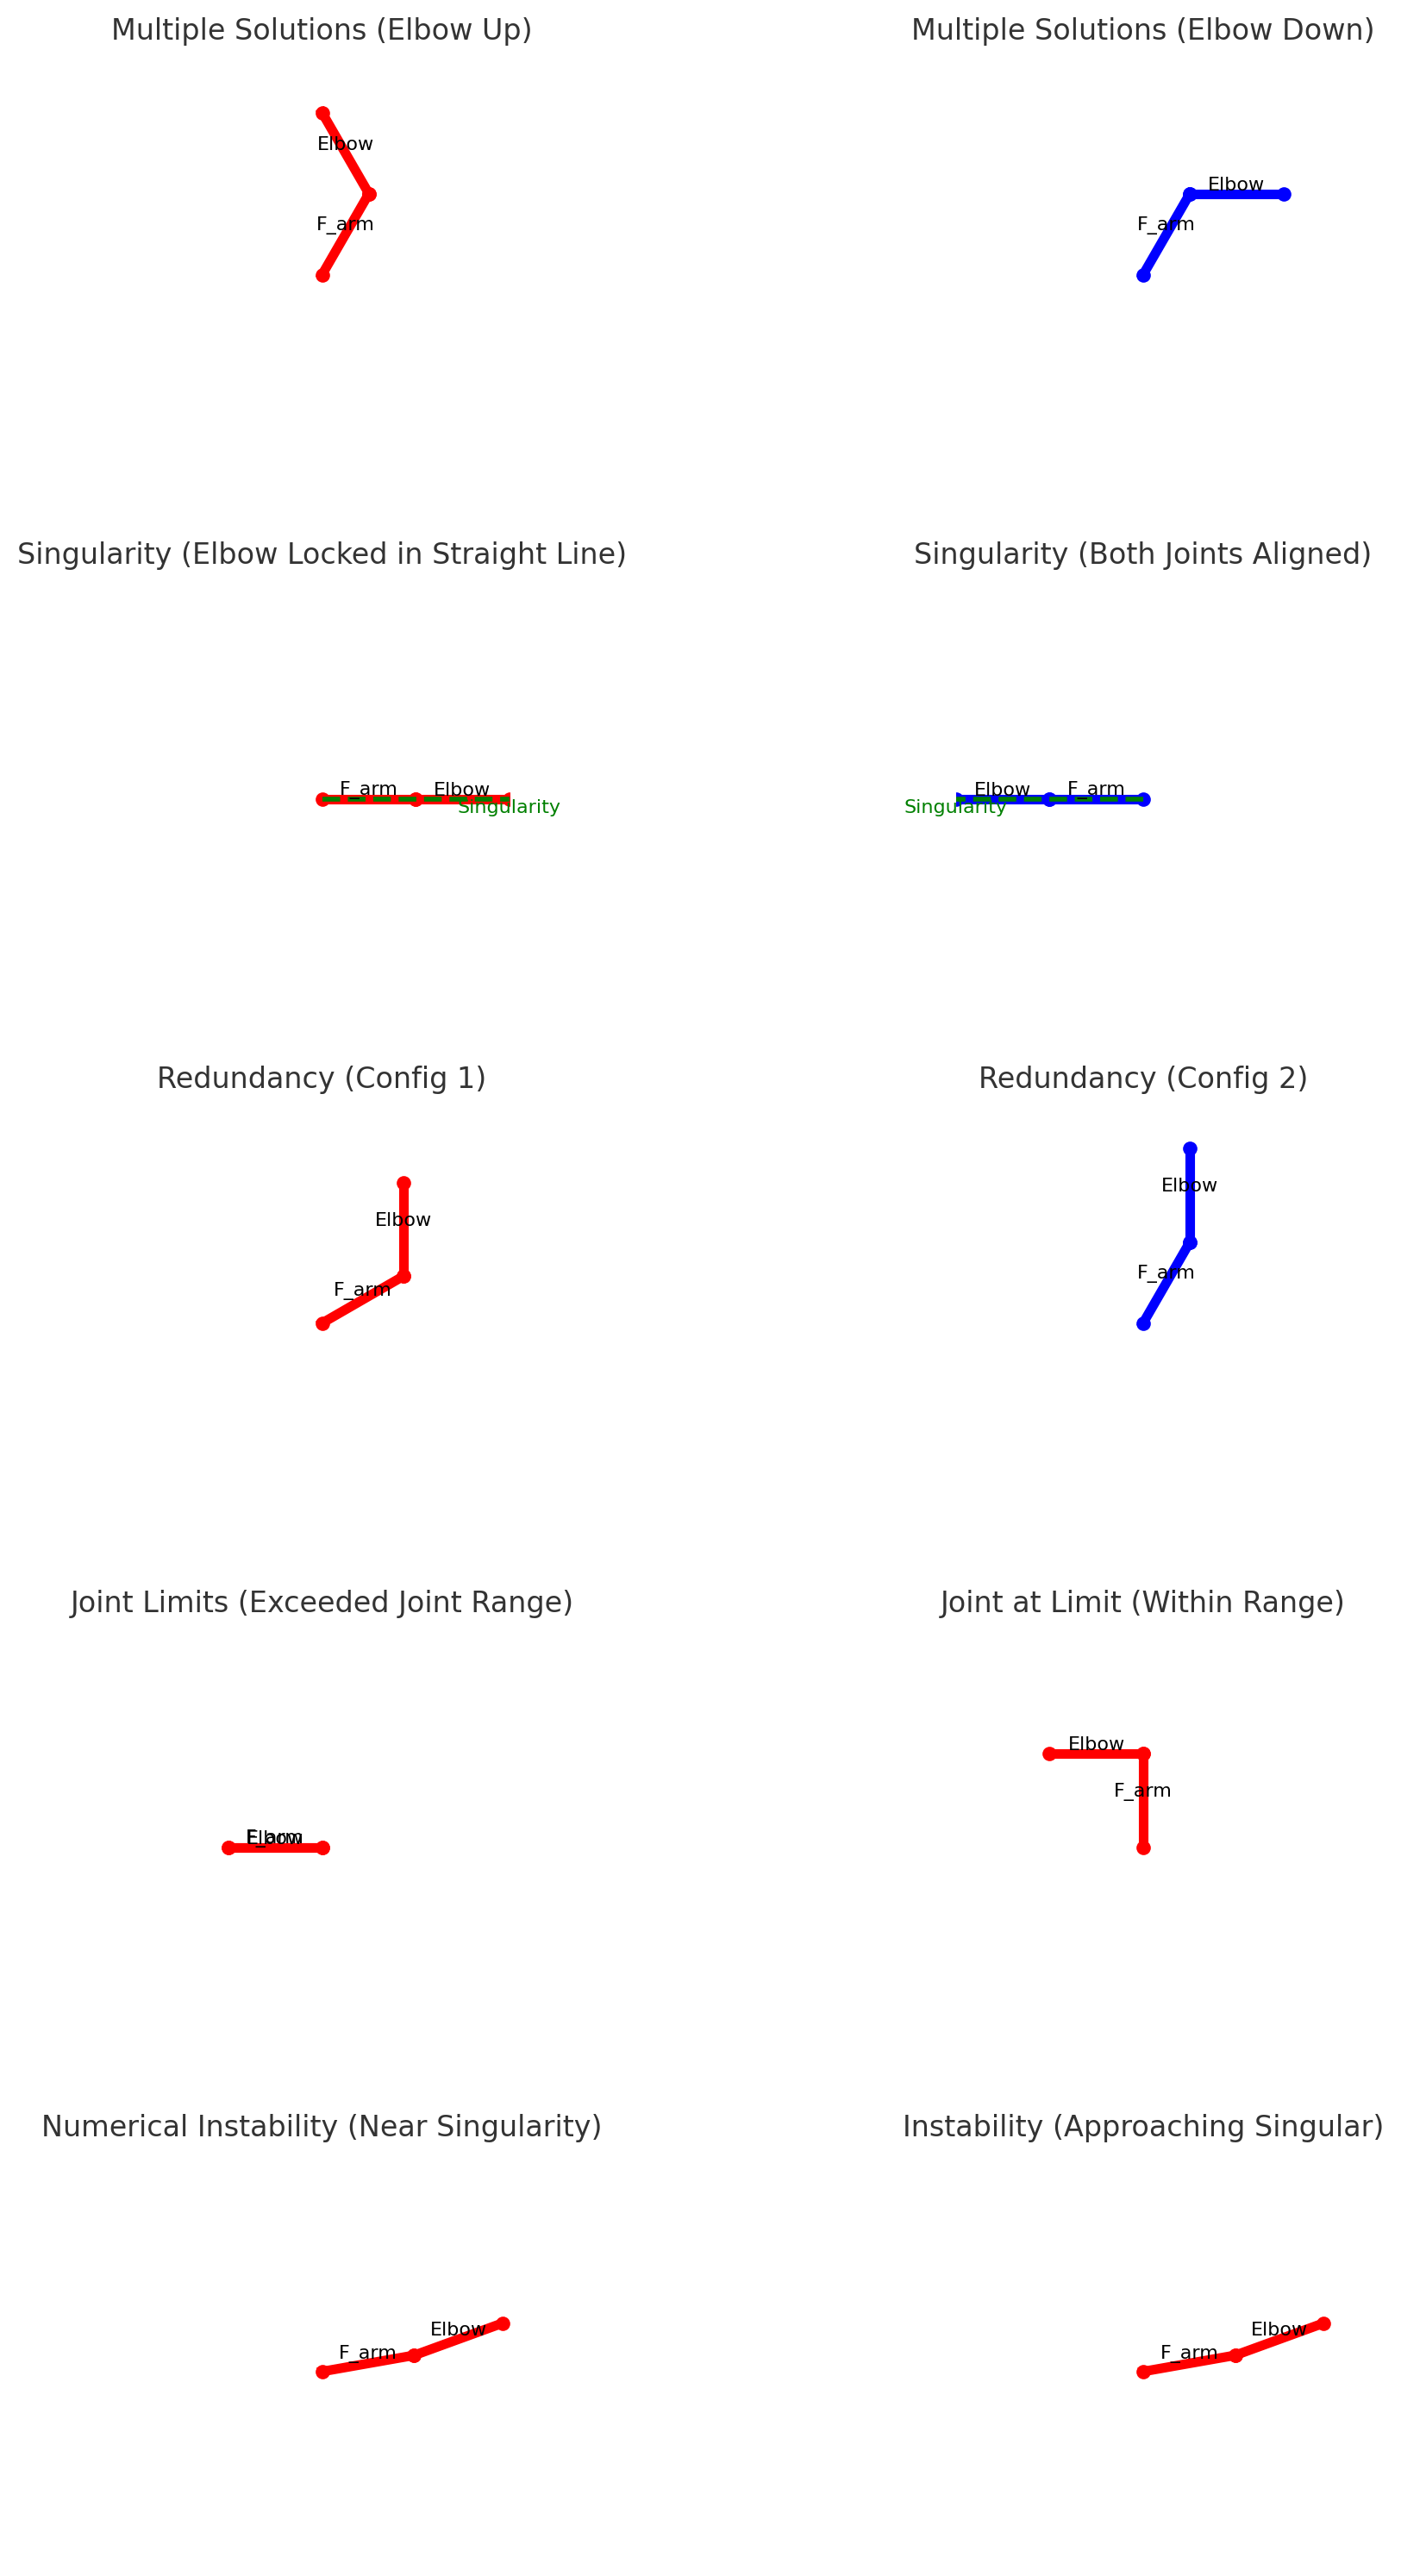
\includegraphics[width = 5in]{chapters/pose_correction/images/problems_classical.png}
  \caption{Problems with classical IK methods}
  \label{fig:problems_classical}
\end{figure}

\subsection{Improved Data-Driven IK Approaches}
\label{ch:pose_correction:related_work:data_driven_ik}
To address the shortcomings of classical IK methods, data-driven approaches have emerged, leveraging large datasets and machine learning to produce more flexible and realistic animations.

\paragraph{Motion Matching} Motion Matching represents a significant shift from traditional techniques by dynamically selecting the most appropriate pose from a large database of motion capture (mocap) data based on user inputs and contextual parameters. Ubisoft's \emph{For Honor} utilized this technique to create more fluid and responsive character animations, as shown in Figure~\ref{fig:for_honor}. Motion Matching's ability to break down animations into fine-grained clips allows for seamless transitions and natural movements.

\begin{figure}
  \centering 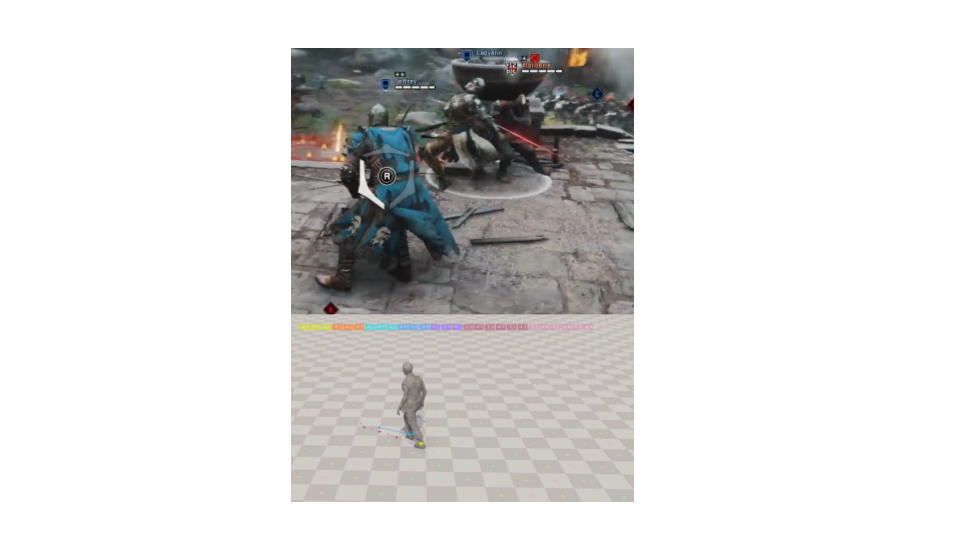
\includegraphics[width = 2.5in]{chapters/pose_correction/images/for_honor.png}
  \caption{Motion Matching in Ubisoft’s \emph{For Honor}}
  \label{fig:for_honor}
\end{figure}

\paragraph{Phase-Functioned Neural Networks (PFNN)} PFNN~\cite{10.1145/3072959.3073663} extends the principles of motion matching by incorporating phase information into the neural network’s weights, allowing the network to generate animations that align with the cyclical nature of bipedal movement (walking, running). Unlike traditional methods that blend animation clips, PFNN encodes the entire animation process within the neural network, providing more control and flexibility, as illustrated in Figure~\ref{fig:pfnn}.

\begin{figure}
  \centering 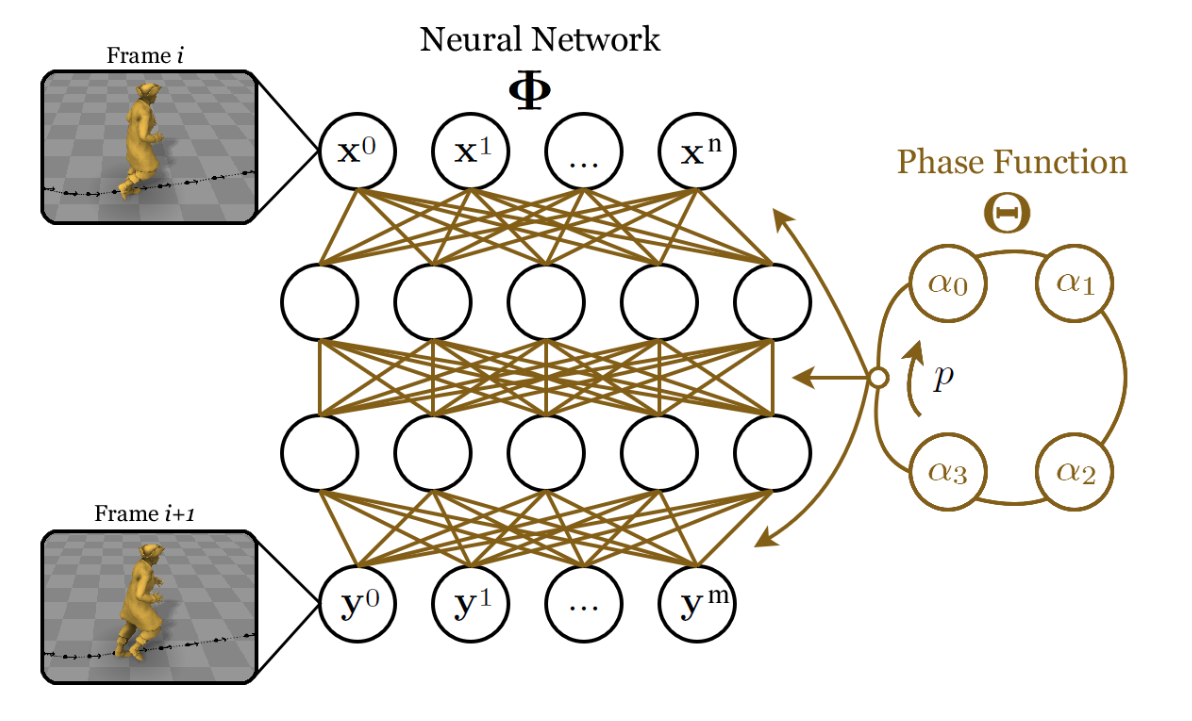
\includegraphics[width = 2.5in]{chapters/pose_correction/images/pfnn.png}
  \caption{Phase-Functioned Neural Networks (PFNN) for motion matching}
  \label{fig:pfnn}
\end{figure}

\paragraph{Style-Based Inverse Kinematics (Style IK)} Style IK~\cite{grochow2004style} leverages machine learning to represent poses in a latent space using Scaled Gaussian Process Latent Variable Models (SGPLVM). By learning the distribution of poses, Style IK generates stylized animations that adhere to aesthetic or functional constraints, making it especially useful in scenarios where mocap data is unavailable or infeasible. Figure~\ref{fig:style_ik} shows how poses are mapped in latent space for Style IK.

\begin{figure}
  \centering 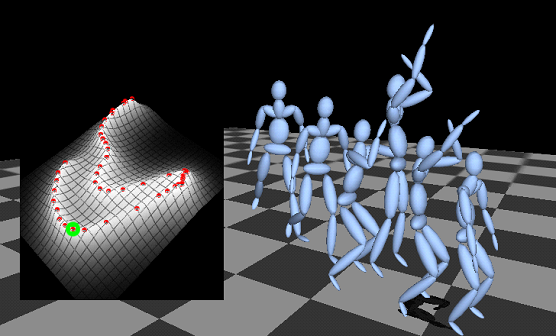
\includegraphics[width = 2.5in]{chapters/pose_correction/images/style_ik.png}
  \caption{Pose in latent space using Style IK}
  \label{fig:style_ik}
\end{figure}

While these data-driven methods resolve many issues inherent to classical IK, they bring challenges like the need for large amounts of training data and increased computational demands, particularly in real-time applications.

\subsection{Latent Space Representations for Pose Generation}
\label{ch:pose_correction:related_work:latent_space}
Latent space representations have become crucial in reducing the complexity of pose and motion data, allowing for more efficient and realistic pose generation and manipulation.

\paragraph{Variational Autoencoders (VAEs) and SMPLify-X} VAEs~\cite{kingma2013auto}, such as those used in SMPLify-X~\cite{pavlakos2019expressive}, learn a probabilistic model of human poses. They can generate and manipulate poses in a lower-dimensional latent space, which can then be sampled to meet specific constraints such as end-effector positions. SMPLify-X is particularly effective in estimating 3D poses from 2D images, as illustrated in Figure~\ref{fig:simplifyx}.

\begin{figure}
  \centering 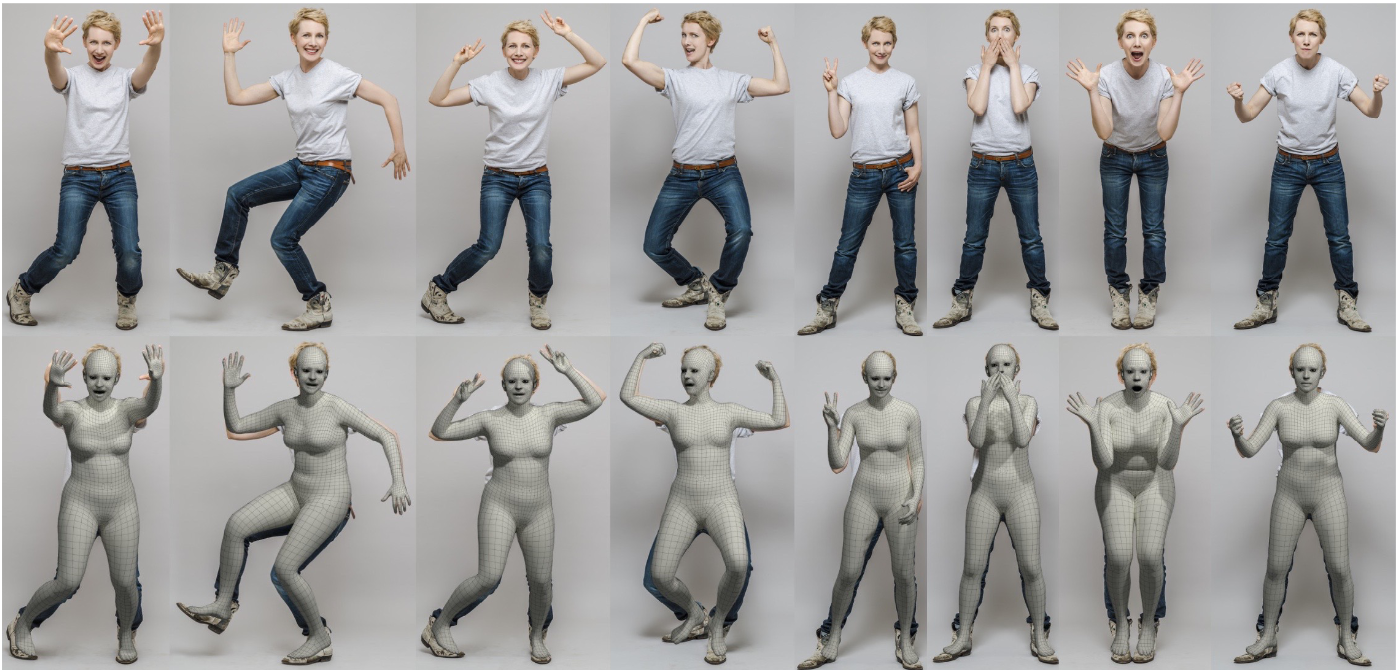
\includegraphics[width = 2.5in]{chapters/pose_correction/images/simplifyx.png}
  \caption{SMPLify-X generating poses from latent space}
  \label{fig:simplifyx}
\end{figure}

\paragraph{VPoser for Pose Correction} VPoser~\cite{pavlakos2019expressive}, a specific implementation of a VAE, encodes human poses into a low-dimensional latent space. This latent space helps regularize pose generation, ensuring that generated poses are realistic and meet specific biomechanical criteria. VPoser plays a critical role in optimization processes by constraining pose generation to physically plausible configurations, as seen in Figure~\ref{fig:vposer}.

\begin{figure}
  \centering \includegraphics[width = 2.5in]{chapters/pose_correction/images/vposer.png}
  \caption{Pose regularization using VPoser in a latent space}
  \label{fig:vposer}
\end{figure}

\subsection{Pose Priors and Corrective Methods}
\label{ch:pose_correction:related_work:pose_priors}
Pose priors provide a mechanism to generate plausible poses based on learned distributions from large datasets. These pose priors ensure that the generated poses are not only valid but also contextually appropriate.

\paragraph{VPoser for Pose Correction in Sign Language Animation} In our system, we utilize VPoser to correct the poses generated by the sign language animation system. By training VPoser on a comprehensive dataset of human poses, we can snap the initial pose to the closest valid pose in the latent space, thereby ensuring realism and accuracy in sign language gestures. This method ensures that the final poses are biomechanically correct and visually appropriate.

\subsection{Conclusion}
\label{ch:pose_correction:related_work:conclusion}
This review has traced the development of IK techniques, from classical methods to data-driven approaches that leverage latent spaces. The incorporation of pose priors, particularly through VPoser, offers a robust solution for pose correction in our sign language animation system, allowing for natural and contextually appropriate movements.

\section{Pose Correction with AZee Low Level synthesis}
\label{ch:pose_correction:pose_correction_with_azee}

In this section, we discuss the application of pose correction techniques to the AZee low-level synthesis system. By integrating pose correction, data-driven IK, and latent space representations into the AZee framework, we aim to enhance the realism and expressiveness of sign language animations.

\subsection{Preparing the dataset}
\label{ch:pose_correction:pose_correction_with_azee:dataset}

The first step in integrating pose correction into AZee is to train a Variational Autoencoder (VAE) on set of sign language poses. For this task, we use a dataset of mocap data collected from the Rosetta dataset~\cite{bertin2022rosetta}. The dataset consists of 167066 poses and should capture the diversity of poses and movements associated with different signs, providing a rich source of training data for the VAE.. Since our focus was only on the upper body, we didn't use the facial bones and the lower body for the training. We also retargeted the mocap data to the BAZeel avatar, which is compatible with the AZee skeleton structure (figure~\ref{fig:retargeted}).

\begin{figure}
  \centering 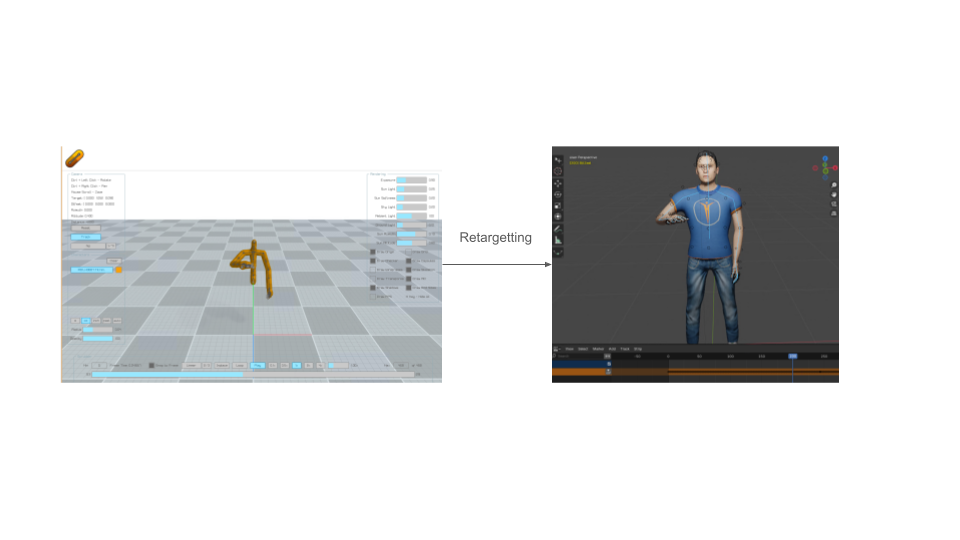
\includegraphics[width = 2.5in]{chapters/pose_correction/images/retargeted.png}
  \caption{Retargeted mocap data to BAZeel avatar}
  \label{fig:retargeted}
\end{figure}

Next, we converted the motion into AZee's FK pose array. The FK pose array consists of the rotation values of each joint in the AZee skeleton (figure~\ref{fig:azee_fk_pose}). This representation is more suitable for the VAE training process, as it captures the pose information in a compact and standardized format.

\begin{figure}
  \centering 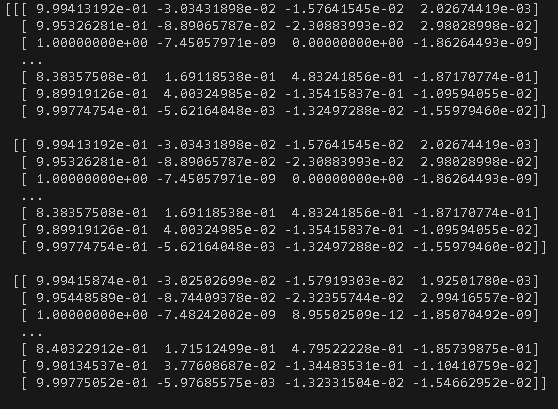
\includegraphics[width = 2.5in]{chapters/pose_correction/images/azee_fk_pose.png}
  \caption{AZee FK Pose Array}
  \label{fig:azee_fk_pose}
\end{figure}

\subsection{Training VPoser}
\label{ch:pose_correction:pose_correction_with_azee:training}

A VAE is a type of generative model that learns a low-dimensional latent space representation of the input data. In the context of character animation, a VAE can be used to capture the distribution of poses in a dataset, allowing for the generation of new poses that are statistically similar to the training data. The VAE consists of an encoder network that maps input poses to a latent space and a decoder network that reconstructs the input poses from the latent space (figure~\ref{fig:vae}).


\begin{figure}[h]
\centering
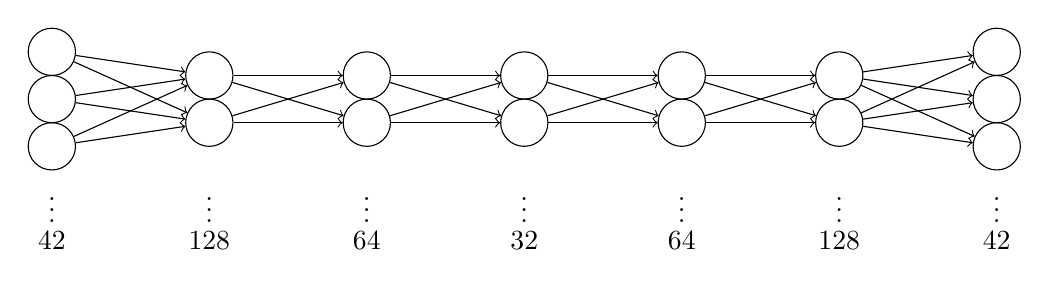
\begin{tikzpicture}[
    every neuron/.style={
        circle,
        draw,
        minimum size=0.6cm
    },
    neuron missing/.style={
        draw=none, 
        scale=1,
        text height=0.333cm,
        execute at begin node=\color{black}$\vdots$
    },
    layer/.style={
        rectangle,
        draw,
        text centered,
        minimum width=2cm
    }
]

% Input Layer
\foreach \i in {1,2,3}
    \node [every neuron/.try, neuron \i/.try] (input-\i) at (0,1.5-\i*0.6) {};

\node at (0,-1) {\vdots};
\node at (0,-1.5) {42};

% Encoder L1
\foreach \i in {1,2}
    \node [every neuron/.try, neuron \i/.try] (L1-\i) at (2,1.2-\i*0.6) {};

\node at (2,-1) {\vdots};
\node at (2,-1.5) {128};

% Encoder L2
\foreach \i in {1,2}
    \node [every neuron/.try, neuron \i/.try] (L2-\i) at (4,1.2-\i*0.6) {};

\node at (4,-1) {\vdots};
\node at (4,-1.5) {64};

% Latent Layer
\foreach \i in {1,2}
    \node [every neuron/.try, neuron \i/.try] (L3-\i) at (6,1.2-\i*0.6) {};

\node at (6,-1) {\vdots};
\node at (6,-1.5) {32};

% Decoder L4
\foreach \i in {1,2}
    \node [every neuron/.try, neuron \i/.try] (L4-\i) at (8,1.2-\i*0.6) {};

\node at (8,-1) {\vdots};
\node at (8,-1.5) {64};

% Decoder L5
\foreach \i in {1,2}
    \node [every neuron/.try, neuron \i/.try] (L5-\i) at (10,1.2-\i*0.6) {};

\node at (10,-1) {\vdots};
\node at (10,-1.5) {128};

% Output Layer
\foreach \i in {1,2,3}
    \node [every neuron/.try, neuron \i/.try] (output-\i) at (12,1.5-\i*0.6) {};

\node at (12,-1) {\vdots};
\node at (12,-1.5) {42};

% Draw the connections
\foreach \i in {1,2,3}
    \foreach \j in {1,2}
        \draw [->] (input-\i) -- (L1-\j);

\foreach \i in {1,2}
    \foreach \j in {1,2}
        \draw [->] (L1-\i) -- (L2-\j);

\foreach \i in {1,2}
    \foreach \j in {1,2}
        \draw [->] (L2-\i) -- (L3-\j);

\foreach \i in {1,2}
    \foreach \j in {1,2}
        \draw [->] (L3-\i) -- (L4-\j);

\foreach \i in {1,2}
    \foreach \j in {1,2}
        \draw [->] (L4-\i) -- (L5-\j);

\foreach \i in {1,2}
    \foreach \j in {1,2,3}
        \draw [->] (L5-\i) -- (output-\j);

\end{tikzpicture}
\caption{Architecture of the VAE}
\label{fig:vae}
\end{figure}

Trained on a dataset containing 167,066 poses. The dataset is divided into training, validation, and test sets, which are loaded using the \texttt{AnimationDS} class from the dataloader. During training, batches of poses are processed, with each batch consisting of 512 samples. The training is carried out on a CUDA-enabled GPU, utilizing mixed precision training for efficiency. The VPoser model architecture consists of a latent space with 32 dimensions (\texttt{latentD}), and the neural network has 512 neurons per layer. 

The loss function used during training includes two primary components: 
\begin{itemize}
    \item \textbf{Reconstruction Loss}: This loss is computed at the joint level by comparing the reconstructed pose with the original pose using L1 loss. An additional pose-level reconstruction loss (L2 loss) is applied during the first 10 epochs to help the model learn better early on.
    \item \textbf{KL Divergence Loss}: The KL divergence regularizes the latent space by enforcing it to follow a standard normal distribution, ensuring that the latent space representation is smooth and continuous.
\end{itemize}

The total loss is the sum of the reconstruction loss and KL divergence loss. The optimization is carried out using the Adam optimizer with a learning rate of $1 \times 10^{-2}$ and weight decay of $0.0001$. A learning rate scheduler is used, which reduces the learning rate by a factor of 0.5 every third of the training epochs. 

\subsection{Implementing Pose Correction}
\label{ch:pose_correction:pose_correction_with_azee:implementation}

With the VAE trained, we can now implement a pose correction system that leverages the learned latent space to match poses generated by the AZee system to the most appropriate pose in the dataset (figure~\ref{fig:pose_correction}).

\begin{figure}
  \centering \includegraphics[width = 2.5in]{chapters/pose_correction/images/pose_correction.png}
  \caption{Pose Correction with VAE}
  \label{fig:pose_correction}
\end{figure}

Algorithm~\ref{alg:pose_correction} outlines the pose correction process. Given a target pose generated by the AZee synthesizor, we first encode the pose into the latent space using the VPoser encoder. We then compute the distance between the encoded pose and each pose in the dataset, selecting the pose with the smallest distance as the best match. Finally, we decode the matched pose back into the AZee FK pose array and apply it to the character.

\begin{algorithm}
  \caption{AZee constraint optimization with pose correction algorithm}
  \label{alg:pose_correction}
  \begin{algorithmic}[1]
  \For{$frame$ \textbf{in} frames}
      \State \texttt{switch\_cursor\_to\_frame($f$)}
      \For{\texttt{parallel\_block \textbf{in} self.parallel\_blocks}}
          \State \texttt{constraints.add(parallel\_block.constraints)}
      \EndFor
      \For{\texttt{constraint \textbf{in} constraints}}
          \State \texttt{constraint.apply($frame$)}
      \EndFor
      \State \texttt{model.pose\_embedding}
      \State \texttt{model.global\_trans}
      \State \texttt{optimizer = \dots}
      \For{\texttt{epoch \textbf{in} range(max\_epochs)}}
          \State \texttt{optimizer.zero\_grad()}
          \State \texttt{\dots}
          \State \texttt{optimizer.step()}
          \If{\texttt{loss.item() < threshold}} \State \texttt{break} \EndIf
      \EndFor
      \State \texttt{posture.keyframe($frame$)}
  \EndFor
  \end{algorithmic}
  \end{algorithm}

\subsection{Results and Evaluation}
\label{ch:pose_correction:pose_correction_with_azee:results}

Snapshots with standard synthesis and synthesis with pose correction and the corresponding AZee code for the same are shown in table~\ref{tab:results}.

\begin{table}
  \centering
  \begin{tabular}{|c|c|c|}
    \hline
    \textbf{Standard Synthesis} & \textbf{Synthesis with Pose Correction} & \textbf{AZee Code} \\
    \hline
    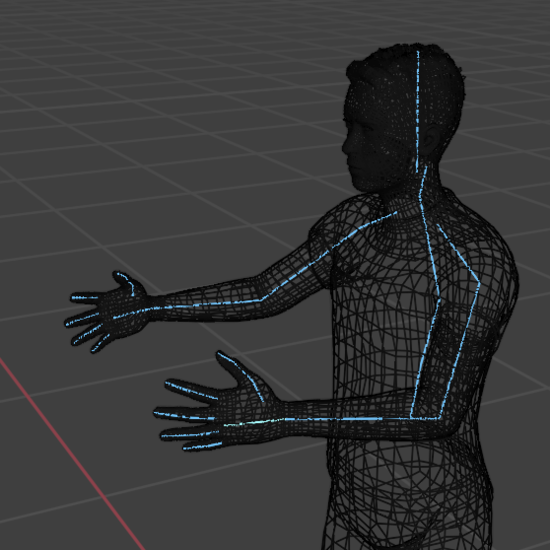
\includegraphics[width = 1.5in]{chapters/pose_correction/images/standard_synthesis_armoire.png} & 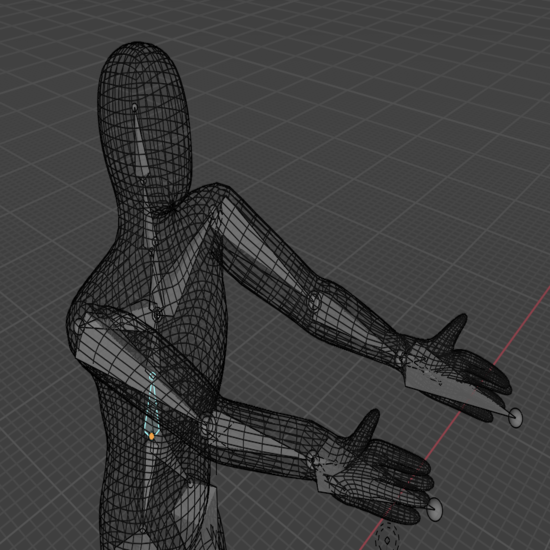
\includegraphics[width = 1.5in]{chapters/pose_correction/images/pose_correction_synthesis_armoire.png} & 
      \emph{:armoire} \\
    \hline
    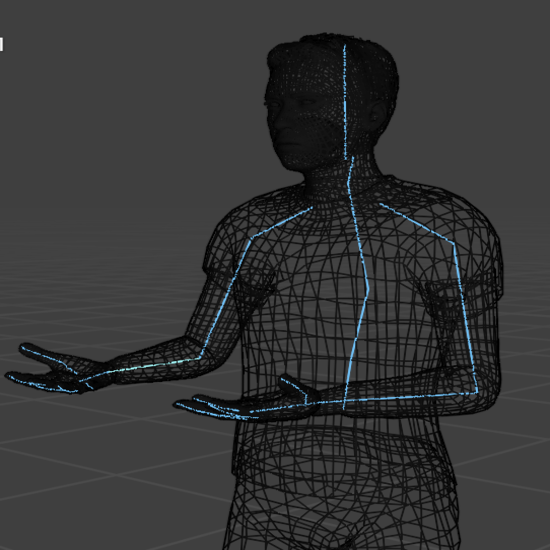
\includegraphics[width = 1.5in]{chapters/pose_correction/images/standard_synthesis_maintenant.png} & 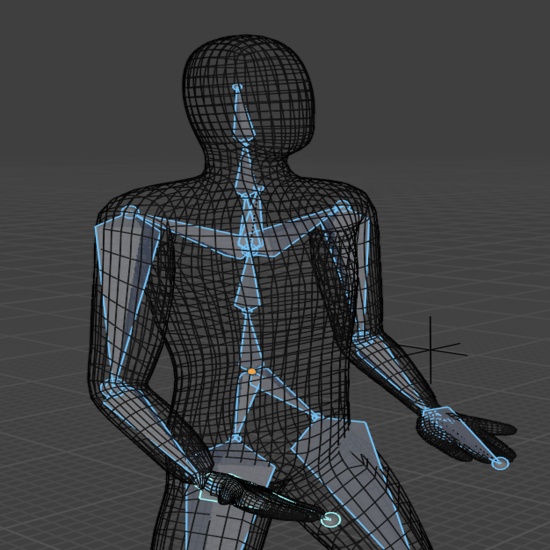
\includegraphics[width = 1.5in]{chapters/pose_correction/images/pose_correction_synthesis_maintenant.png} &
      \emph{:maintenant} \\
    \hline
    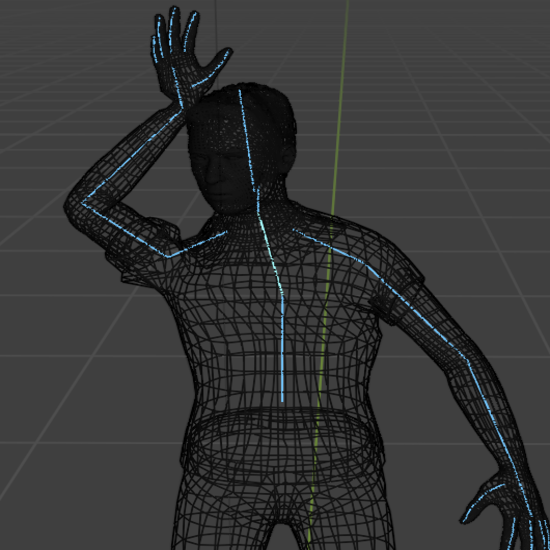
\includegraphics[width = 1.5in]{chapters/pose_correction/images/standard_synthesis_abt_ref_irak.png} & 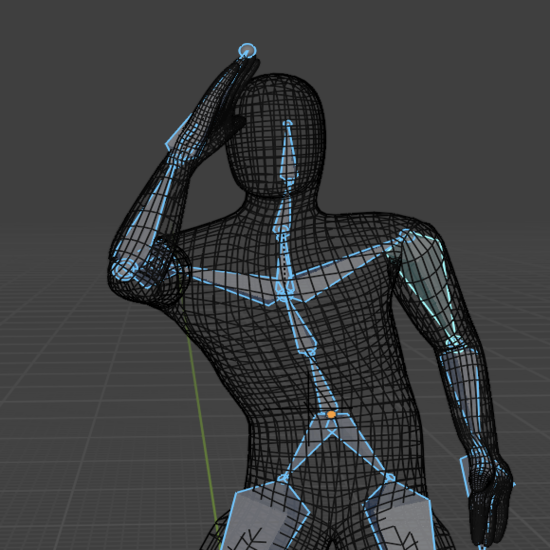
\includegraphics[width = 1.5in]{chapters/pose_correction/images/pose_correction_synthesis_abt_ref_irak.png} &
      \emph{:about-ref(:irak, Rssp)} \\
    \hline
  \end{tabular}
  \caption{Comparison of standard synthesis and synthesis with pose correction}
  \label{tab:results}
\end{table}

The synthesized videos can also be viewed at \href{todo}.

Initial subjective evaluations suggest that the pose correction system produces more natural and contextually appropriate animations compared to standard joint-limit based synthesis. However, due to retargeting losses, the integration of pose correction into Sign Language synthesis is still in the early stages. We also observe that the corrector might change the pose of the character in a way that is not always desirable~\ref{fig:problem_pose_correction}.

\begin{figure}
  \centering 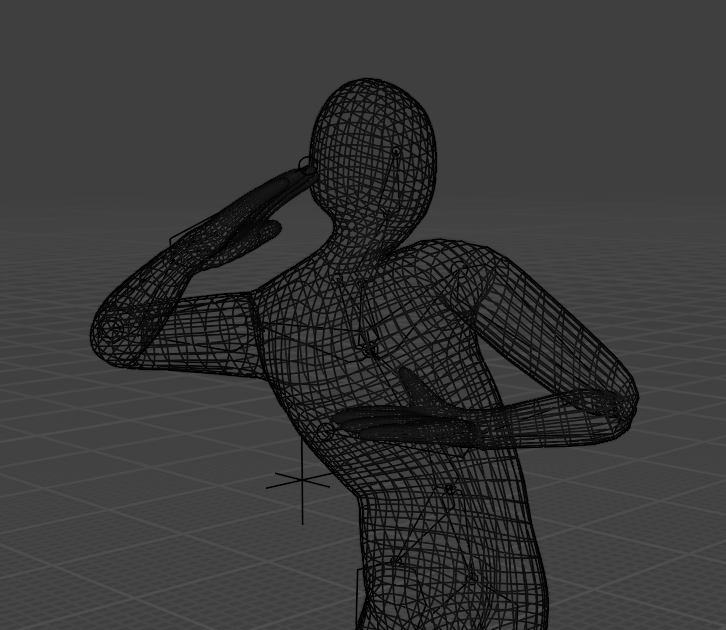
\includegraphics[width = 2.5in]{chapters/pose_correction/images/problem_pose_correction.png}
  \caption{Problems with current correction module}
  \label{fig:problem_pose_correction}
\end{figure}

Lastly, figure~\ref{fig:losses} shows how retargeting the mocap data to the AZee skeleton structure results in a loss of information. This loss can affect the quality of the generated animations and is an area for future improvement.

\begin{figure}
  \centering 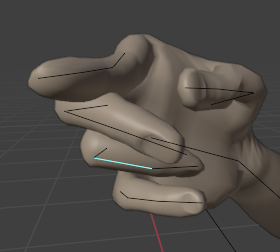
\includegraphics[width = 2.5in]{chapters/pose_correction/images/losses.png}
  \caption{Losses in retargeting mocap data}
  \label{fig:losses}
\end{figure}

\section{Discussion}
\label{ch:pose_correction:discussion}

The integration of pose correction into the AZee system represents a significant advancement in sign language synthesis. By leveraging data-driven IK and latent space representations, we are able to generate more realistic and contextually appropriate sign language animations. This has the potential to enhance the expressiveness and naturalness of sign language avatars, making them more engaging and accessible to users. In some ways, this offfers a new perspective to Sign Language synthesis where the linguistics decides the "what" and the pose corrector decides the "how" of the animation.

For future, posers based on neural distance fields~\cite{tiwari2022pose} or diffusion~\cite{lu2023dposer} could be used for pose correction since the current poser has a bayesian bias. Also, continuity of the trained model with respect to signing spaces could be studied further improving the the learnt pose prior.

While the integration of deep learning into SL synthesis offers numerous advantages, it also introduces new challenges. Data-driven and latent space methods typically require significant computational resources, both during training and inference. This can be a major barrier in real-time applications, where low latency is critical. Also the effectiveness of deep learning models depends heavily on the availability of high-quality training data. In many cases, obtaining sufficient mocap data can be difficult, especially for non-standard or stylized animations. Lastly, while deep learning models can generate realistic and high-quality animations, they often lack the fine-grained control that human animators require. Ensuring that these models produce outputs that align with artistic vision remains a significant challenge.

\end{document}